% Desarrollo
\chapter{Desarrollo} \label{chap:desarrollo}
	En este cap'itulo se describe de manera detallada todo el proceso de desarrollo de este proyecto de pasant'ia. Para ello, se va a describir como fueron desarrolladas cada una de las fases involucradas.

\section{Fase 1: Preparaci'on Previa}
	Durante esta fase se realizaron diferentes reuniones organizadas por la tutora industrial con el fin de tener un entrenamiento en el software SAP. Para ello, distintos empleados de la compa\~n'ia estuvieron en dichas reuniones para dictar los talleres.
	Los talleres recibidos fueron acerca de los siguientes m'odulos:
\begin{itemize}
\item M'odulo de Gesti'on de Calidad (QM)
\item M'odulo de Gesti'on de Materiales (MM)
\item M'odulo de Gesti'on Financiera (FI)
\item M'odulo de Controlling (CO)
\item M'odulo de Ventas y Distribuci'on (SD)
\end{itemize}
	Para cada m'odulo fueron explicados los conceptos b'asicos que est'an involucrados en cada uno. Espec'ificamente en el taller de Ventas y Distribuci'on (SD), se explic'o el ciclo de ventas general. Para ello, la persona encargada, explic'o por detalle cada una de las etapas por las cuales pasa un proceso de ventas en general (Realizaci'on del Pedido de Ventas, Entrega, Facturaci'on). 
	Adicionalmente, fue impartido un taller sobre el lenguaje de Programaci'on ABAP/4, para conocer un poco acerca de la estructura del lenguaje. Durante este taller, se recibieron conocimientos acerca de: estructuras de control, herramientas que posee el lenguaje para emitir reportes como por ejemplo: smartforms, que son una especie de formulario que se pueden imprimir. 
	Adem'as, se recibi'o material acerca de otro template que fue desarrollado para otro tipo de industria, pero que sirvi'o como base para ver como el m'odulo de Ventas y Distribuci'on es puesto en pr'actica, y para servir como ejemplo a la hora de implantar dicho m'odulo a la empresa de bebidas de consumo masivo.
	
\section{Fase 2: Business Blueprint}
	Durante esta fase fueron desarrolladas las siguientes actividades:
\begin{itemize}
\item Identificar el proceso de Master Data (Datos Mestros) a desarrollar en SAP.
\item Identificar el proceso de Sales (Pedidos de Venta) a desarrollar en SAP.
\item Identificar el proceso de Shipping and Transportation (Embarque y transporte) a ser desarrollado en SAP.
\item Identificar el proceso de Billing (Facturaci'on) a ser desarrollado en SAP.
\end{itemize}

	Como fue explicado en el cap'itulo anterior, en esta fase se detallan cada uno de los procesos del negocio de la compa\~n'ia para la cual se est'a llevando el proyecto; esto involucra conocer los procesos actuales y como se podr'ian aplicar dichos procesos en SAP. 
	
	Para el caso de la empresa de bebidas de Consumo Masivo para la cual se est'a trabajando, se van a analizar cada uno de los procesos involucrados en Ventas y Distribuci'on, para ello, se proceder'a en las sub-secciones siguientes a detallar cada una de las actividades mencionadas en la lista anterior.
	
\subsection{Identificaci'on del proceso de Master Data (Datos Maestros)}
	En esta actividad, los datos maestros que fueron estudiados e identificados para el caso de la empresa de bebidas de consumo masivo para la cual se est'a realizando esta configuraci'on, consistieron en los datos que forman parte de la estructura organizativa de la empresa. Para ello se realiz'o un estudio con otras empresas que manejan el mismo rubro para saber cu'al es el camino a seguir. En el siguiente gr'afico se muestra la organizaci'on de SSA BEVERAGE:
\begin{figure}[htb]
\centering
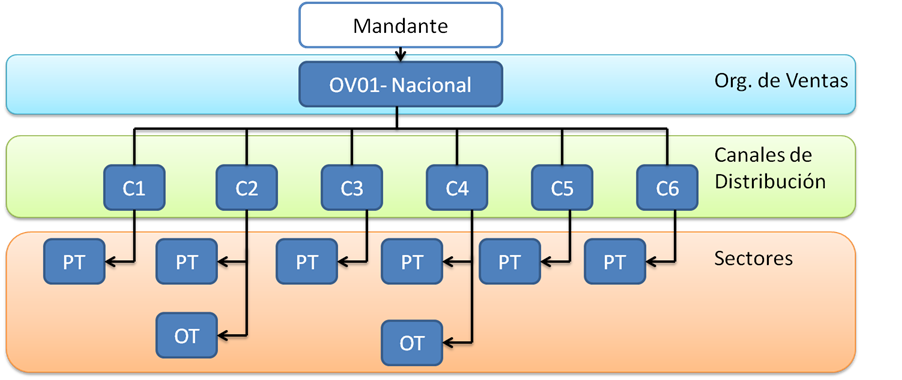
\includegraphics[scale=0.45,type=png,ext=.png,read=.png]{figures/Org1}
\caption{Estructura de la Enpresa definida para el M'odulo SD (Parte 1)}
\label{fig:estructura}
\end{figure}

\begin{figure}[htb]
\centering
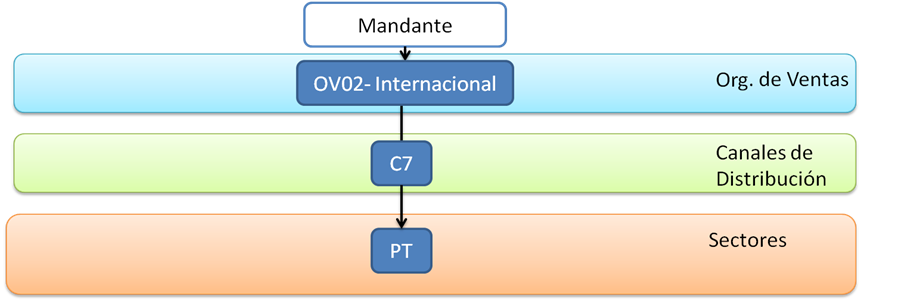
\includegraphics[scale=0.45,type=png,ext=.png,read=.png]{figures/Org2}
\caption{Estructura de la Empresa definida para el M'odulo SD (Parte 2)}
\label{fig:estructura}
\end{figure}

	Para las Organizaciones de Ventas, se fijaron dos para configurar en la siguiente etapa, y son las que se muestran en la siguiente lista:

\begin{itemize}

\item Nacional: Se va a encargar de atender a los clientes nacionales
\item Internacional : Se va a encargar de atender las exportaciones de los productos
\end{itemize}
	Luego se definieron los Canales de Distribuci'on. Para este caso, se decidi'o fijar 7 canales de distribución. Estos son los que se listan en la siguiente lista:

\begin{itemize}
\item Distribuci'on Directa: Este canal ser'a utilizado para atender a los clientes en general.
\item Intermediario: Este canal ser'a utilizado para atender a aquellos clientes que tengan alg'un intermediario con el que a trav'es de ellos realicen alguna compra de materiales.
\item Eventos: Este canal ser'a utilizado para captar clientes a trav'es de eventos que realice la compa\~nia. 
\item Institucionales: Esta canal ser'a empleado para atraer a clientes a trav'es de instituciones sin fines de lucro.
\item Mayoristas: Este canal ser'a empleado para atraer a aquellos clientes se compren al mayoreo.
\item Traslados: Este canal ser'a utilizado para aquellos clientes que est'en a lo largo del pa'is.
\item Exportaciones: Este canal ser'a utilizado para aquellos clientes que est'en en el exterior.
\end{itemize}
	A continuaci'on, se procedi'o a establecer los sectores en los cuales ser'an agrupados los materiales a producir, como se muestra en la siguiente lista:
\begin{itemize}
\item Producto Terminado: Consiste en el grupo conformado por todas aquellas bebidas que vayan a ser vendidas por la empresa, que ya han sido elaboradas.
\item Otros: En este grupo entran aquellos materiales que fueron usados para la elaboraci'on de los productos finales, del cual qued'o un remanente, como por ejemplo, del mosto sobrante de la elaboraci'on de la cerveza.
\end{itemize}

Luego se procedi'o a establecer varias oficinas de ventas. Para esto, se decidi'o mantener la misma distribuci'on de los Centros de Distribuci'on que fueron colocados dentro del m'odulo de Gesti'on de Materiales (MM), en la cual se dividi'o al territorio en varias regiones. Luego, se defini'o una oficina por cada regi'on, quedando las mismas de la siguiente manera:
\begin{itemize}
\item Capital
\item Central
\item Los Llanos
\item Nororiental
\item Insular
\item Occidental
\item Andes
\item Zuliana
\end{itemize}
	Posteriormente, se hizo la identificaci'on de los puestos de expedici'on por cada centro de distribuci'on. Dada la distribuci'on de las ofcinas de ventas en el p'arrafo anterior, y que las mismas presentan una distribuci'on equivalente a los Centros de Distribuci'on, se decidi'o establecer dos puestos de carga por cada uno, como se muestra a continuaci'on:
\begin{itemize}
\item Despacho: Este puesto se encarga de la entrega de los materiales a los clientes.
\item Retorno: Este puesto se encarga de recibir aquellos materiales que son enviados por los clientes, como por ejemplo: botellas retornables, etc.
\end{itemize}
	Para establecer los puestos de expedici'on en la siguiente etapa, fueron identificados dos puestos de carga por cada puesto de expedici'on.
\subsection{Identificaci'on del proceso de Sales (Pedidos de Ventas)}
	Dentro del proceso de ventas que es manejado por el m'odulo SD,'este es el punto de partida, ya que el primer paso para poder realizar el ciclo de una venta de un material es la realizaci'on de un Pedido de Ventas. Para ello, es creado un documento de Pedido de Ventas que contiene varios tipos de informaci'on, como por ejemplo:
\begin{itemize}
\item Informaci'on personal del cliente
\item Informaci'on del(los) material(es) a adquirir
\item Informaci'on sobre las condiciones de pago
\end{itemize}
	Para ello, es necesario identificar dos puntos importantes en esta etapa:
\begin{itemize}
\item Tipo de Pedido a realizar: Representa el tipo de Documento a crear
\item Clases de Mensajes: Contiene las rutinas de impresi'on de documentos
\item Tipos de Posici'on: Cada rengl'on del documento relacionado con cada material representa una posici'on del documento
\item Clases de condici'on: Como su nombre lo indica, son condiciones. 'Estas son establecidas a los precios de los productos
\item Esquemas de C'alculo: Contiene las clases de Condici'on a utilizar
\end{itemize}
	Para este proyecto, se decidi'o utilizar el Pedido Est'andar, el cual permite realizar un pedido normal. Para las clases de mensajes se decidi'o adoptar la est'andar, al igual que los tipos de posici'on y las clases de condici'on.
\subsection{Identificaci'on del proceso de Shipping and Transportation (Embarque y Transporte)}
	El segundo paso dentro del ciclo general de una venta en SAP es el proceso de Entega (Shipping), el cual consiste en generar un Documento de Entrega, en el cual consta, adem'as de los datos provenientes del Documento de Ventas al cual hace referencia, los datos relacionados con el puesto de expedici'on en el cual ser'a entregado el material solicitado. Para esto es necesario definir el tipo de Documento a utilizar. 
	Dado que en el segmento anterior se decidi'on definir un Pedido Est'andar, para esta parte del ciclo de Ventas se decidi'o definir un Documento de Entrega Est'andar, ya que es el que corresponde con el tipo de pedido establecido anteriormente.

\subsection{Identificaci'on del proceso de Billing (Facturaci'on)}
	El tercer y 'ultimo paso dentro del ciclo general de una venta en SAP es el proceso de Facturaci'on (Billing). Para este caso se define un tipo de documento de Facturaci'on acorde con el tipo de Pedido de Ventas y tipo de Entrega definidos anteriormente.
	Para el pedido Estandar definido m'as atr'as, fueron definidos dos tipos de Documentos de Facturaci'on: El primero, la Facturaci'on Est'andar, el cual es utilizado para crear la factura de un pedido existente, para as'i cerrar el ciclo normal de la venta de un material. El segundo, consiste en la \textbf{Anulaci'on de Factura}, 'este es usado para una vez que haya sido creada la factura de un pedido, y halla ocurrido alg'un problema durante el proceso en el cual fue realizado dicho pedido, el mismo se pueda anular, y as'i se pueda volver a crear.

\section{Fase 3: Realizaci'on (Construcci'on y Pruebas)}
	Las actividades desarrolladas en esta fase se dividieron en dos grupos principales: Configuraci'on Base del M'odulo de Ventas y Distribuci'on (SD) para SSA Beverage y Elaboraci'on de las facturas legales.
	A continuaci'on, se proceder'a a detallar cada uno de los dos grupos.
\subsection{Configuraci'on Base del M'odulo de Ventas y Distribuci'on para SSA Beverage}
	Para poder realizar las configuraciones, hubo que dividirlas en varios grupos, los cuales se muestran a continuaci'on:
\subsubsection{Configuraci'on de la parte organizativa de la Empresa}
	Este grupo fue compuesto por las configuraciones realizadas para definir la estructura de SSA Beverage. Para ello, se ingres'o a SAP, y a trav'es del Customizing, fue posible efectuarlas. Se comenz'o configurando las Organizaciones de Ventas, Canales de Distribuci'on y Sectores definidos en la fase anterior. A continuaci'on, se muestran figuras de las tres configuraciones realizadas:
	
\begin{figure}[htb]
\centering
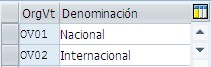
\includegraphics[scale=0.65,type=jpg,ext=.jpg,read=.jpg]{figures/OrgVentas}
\caption{Organizaciones de Ventas definidas para el M'odulo SD}
\label{fig:orgventas}
\end{figure}
\begin{figure}[htb]
\centering
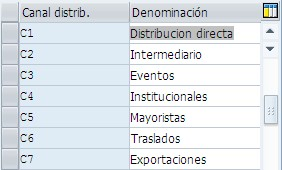
\includegraphics[scale=0.65,type=jpg,ext=.jpg,read=.jpg]{figures/CanalesDistribucion}
\caption{Canales de Distribuci'on definidos para el M'odulo SD}
\label{fig:canales}
\end{figure}
\begin{figure}[htb]
\centering
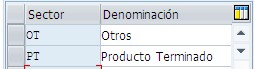
\includegraphics[scale=0.65,type=jpg,ext=.jpg,read=.jpg]{figures/Sectores}
\caption{Sectores definidos para el M'odulo SD}
\label{fig:sectores}
\end{figure}




\section{Fase 4: Presentaci'on y Resultados Finales}
Aqui iran los resultados finales